\clearpage

\lehead[]{\normalfont\sffamily\hspace*{-2.00cm}\textcolor{white}{\colorbox{lightblue}{\parbox[c][0.70cm][b]{1.60cm}{
\makebox[1.60cm][r]{\thechapter}\\ \makebox[1.60cm][r]{ÜBUNG}}}}\hspace{0.17cm}\textcolor{lightblue}{\chaptertitle}}
\rohead[]{\textcolor{lightblue}{\chaptertitle}\normalfont\sffamily\hspace*{0.17cm}\textcolor{white}{\colorbox{lightblue}{\parbox[c][0.70cm][b]{1.60cm}{\thechapter\\
ÜBUNG}}}\hspace{-2.00cm}}
%\chead[]{}
\rehead[]{\textcolor{lightblue}{AvHG, Inf, My}}
\lohead[]{\textcolor{lightblue}{AvHG, Inf, My}}

\section{Rekursion: Programmieraufgaben}

Erzeuge in deinem eigenen Projekt ein neues Java-Package mit dem Namen
\myPackage{rekursion}. Kopiere anschließend die Datei \myFile{Rekursion1.java}
aus dem Kurs-Repository in das gerade angelegte Package in deinem Projekt und bearbeite
die Aufgaben dort.

\subsection{Aufgabe 1: Berechnung der Fakultät}

In der Wahrscheinlichkeitsrechnung benutzt man sehr häufig die Fakultätsfunktion, die rekursiv definiert ist:

$0! = 1$ \hspace{2cm}		(0! wird „0 Fakultät“ gesprochen)

$n! = n \cdot (n-1)!$

Programmiere eine Java-Methode \lstinline|fakultaet()|, die n als Parameter
erhält und die Fakultät von n zurück gibt (beides sollen ganze Zahlen sein).
Kommentiere anschließend in der Datei den Aufruf der Methode unterhalb des
Kommentars \glqq\lstinline|// Aufgabe 1|\grqq\ aus und teste die Methode.


\subsection{Aufgabe 2: Zweier-Potenzen}

Die Zahlenfolge 1, 2, 4, 8, 16, \ldots lässt sich folgendermaßen rekursiv
definieren (bitte selber überlegen und eintragen):

zahlenfolge(0) = 

zahlenfolge(n) =

\begin{tabular}{|c|c|c|c|c|c|}\hline
\textbf{n}              & 0 & 1 & 2 & 3 &  4 \\ \hline
\textbf{zahlenfolge(n)} & 1 & 2 & 4 & 8 & 16 \\ \hline
\end{tabular}

Programmiere eine Java-Methode \lstinline|zahlenfolge()|, die n als Parameter
erhält und das Ergebnis der Folge für n zurück gibt (beides sollen ganze Zahlen sein). 
Kommentiere anschließend in der Datei den Aufruf der Methode unterhalb des
Kommentars \glqq\lstinline|// Aufgabe 2|\grqq\ aus und teste die Methode.


\subsection{Aufgabe 3: Papierformate}

Hast du dich schon einmal gefragt, warum wir eigentlich meist auf A4-Blättern
schreiben? Papier könnte ja irgendein beliebiges Format haben. Es könnte
quadratisch sein, es könnte 20 x 25 cm groß oder 10 x 30 cm groß sein. Aber
nein, unser Papier (auch das, welches du gerade liest), ist eben meist DIN A4,
also 21,0 x 29,7 cm groß.

Früher war das nicht so. Jede Person, die Papier herstellte, schnitt es
irgendwie zu: gerade so, wie es ihr passte. Diese Tatsache bereitete vielen
Leuten Mühe, etwa den Sekretärinnen, deren Briefpapiere nie in irgendwelchen
Couverts Platz fanden.

Einige praktische Köpfe nahmen sich deshalb vor, ein für allemal aufzuräumen
mit diesem Papier-Durcheinander. Man erfand die DIN-Norm 472 (DIN = Deutsche
Industrie Norm). Darin wurde festgelegt, in welchen Größen die Papierbögen
herzustellen und zu gebrauchen sind. Zuerst wurde das größte Papierformat
festgelegt. Man nannte es A0 und definierte folgendes:

\begin{quotation}
\noindent Ein A0 Papierbogen ist 1 m² groß und sein Seitenverhältnis beträgt 1 :
$\sqrt{2}$. Dies führt zu einer Länge von 118,9 cm und einer Breite von 84,1
cm.
\end{quotation}

Die weiteren Formate wurden wie folgt festgelegt:

\begin{quotation}
\noindent Das Papierformat A1 erhält man, indem man ein A0 Blatt so faltet,
 dass seine Breitseiten aufeinander zu liegen kommen.

\vspace{3mm}

\noindent Auf dieselbe Weise -- durch wiederholtes Falten -- erhält man die
weiteren Papierformate der DIN-A-Reihe.
\end{quotation}

Für alle Formate außer A0 gilt also: 
Die Höhe ist genau so groß wie die Breite des nächstgrößeren Formats und die
Breite entspricht der halben Höhe des nächstgrößeren Formats.

Programmiere eine Java-Methode \lstinline|breite()|, die die Breite eines
Papierformats als Fließkommazahl zurück gibt. Programmiere eine Java-Methode
\lstinline|hoehe()|, die die Höhe eines Papierformats als Fließkommazahl zurück
gibt.

Beide Methoden sollen die Nummer des Papierformats (0 bis 6) als Parameter
erhalten. 

Kommentiere anschließend in der Datei die Aufrufe der Methoden unterhalb des
Kommentars \glqq\lstinline|// Aufgabe 3|\grqq\ aus. Teste die Methoden und
fülle die Tabelle aus:

\bgroup
\def\arraystretch{1.2}
\begin{tabular}{|c|c|c|c|c|c|c|c|}\hline
\textbf{Format}       & \textbf{A0} & \textbf{A1} & \textbf{A2} & \textbf{A3} & \textbf{A4} & \textbf{A5} & \textbf{A6} \\ \hline
\textbf{Breite in cm} &  84,1 &  &  &  & 21,0 & & \\ \hline
\textbf{Höhe in cm}   & 118,9 &  &  &  & 29,7 & & \\ \hline
\end{tabular}
\egroup


\section{Rekursion mit Turtle-Grafik}

Figuren, bei denen im Kleinen die gleiche Struktur wie im Großen auftritt,
nennt man \emph{Fraktale}.

Für die folgenden Aufgaben kopierst du dir die Datei
\myFile{Rekursion2.java} aus dem Kurs-Repository in dein eigenes Projekt (und
dort in das bereits existierende Package \myPackage{rekursion}).

\subsection{Aufgabe 1: Binärer Baum}

Programmiere eine Methode

\begin{lstlisting}
public void baum(double laenge, int stufen)
\end{lstlisting}

die einen Binären Baum mit der angegebenen Anzahl Stufen zeichnet. Der Aufruf
der Methode mit der im Textfeld eingegebenen Stufenzahl braucht im Code nur
noch auskommentiert werden. Der Parameter \lstinline|laenge| gibt die Länge des
untersten Astes an. Von jedem Ast gehen zwei kleinere Äste im Winkel von +45°
und –45° ab. Die Länge der Ästen beträgt 6/10 der aktuellen Astlänge. In den
nachfolgenden Abbildungen siehst du wie ein Baum rekursiv entsteht:

\begin{minipage}[b]{0.25\textwidth}
  \centering
  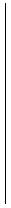
\includegraphics[width=0.04\textwidth]{./inf/SEKII/06_Java_Rekursion/Aufgabe2_1-1.png}
  \captionof{figure}{Stufe 1}
\end{minipage}\hfill                  
\begin{minipage}[b]{0.3\textwidth}
  \centering
  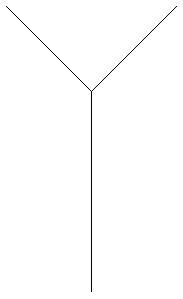
\includegraphics[width=0.55\textwidth]{./inf/SEKII/06_Java_Rekursion/Aufgabe2_1-2.png}
  \captionof{figure}{Stufe 2}
\end{minipage}\hfill
\begin{minipage}[b]{0.3\textwidth}
  \centering
  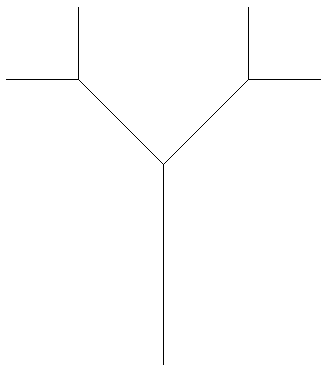
\includegraphics[width=1.0\textwidth]{./inf/SEKII/06_Java_Rekursion/Aufgabe2_1-3.png}
  \captionof{figure}{Stufe 3}
\end{minipage}

\vspace{5mm}

\begin{minipage}[b]{1.0\textwidth}
  \centering
  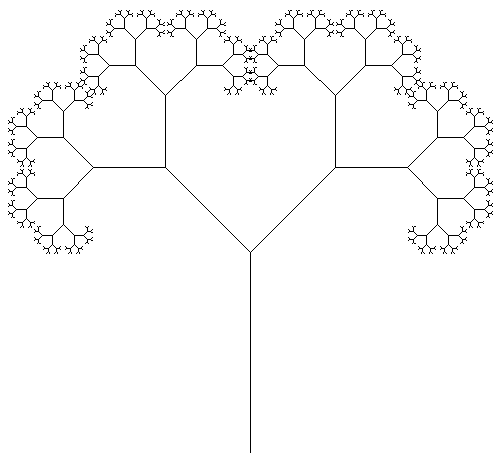
\includegraphics[width=0.5\textwidth]{./inf/SEKII/06_Java_Rekursion/Aufgabe2_1-10.png}
  \captionof{figure}{Ein Binärer Baum der Stufe 10}
\end{minipage}

Lösungsansatz:

Die Turtle soll einen Baum mit einer beliebigen Stufenanzahl zeichnen. Falls
die Stufenanzahl größer als 0 ist, geht sie dazu folgendermaßen vor:

Sie geht um die angegebene Länge vorwärts, dreht sich nach links und zeichnet
rekursiv einen Baum, der eine Stufe kleiner ist. Dann dreht sie sich nach
rechts und zeichnet auch dort rekursiv einen Baum, der eine Stufe kleiner ist.
Sie dreht sich wieder so, dass sie nach oben blickt, und läuft dann mit
\lstinline|t.vor(-laenge)| rückwärts zu ihrem Ausgangspunkt zurück.


\subsection{Aufgabe 2: Farnwedel}

Programmiere eine Methode

\begin{lstlisting}
public void farnwedel(double laenge, int stufen)
\end{lstlisting}

die auf ähnliche Weise arbeitet wie die Methode der vorhergehenden Aufgabe. Der
„Baum“ ist jetzt jedoch nicht mehr binär, sondern hat drei Äste, die in
unterschiedlichen Winkeln abzweigen. Der linke und der rechte Ast besitzen 1/2
der Länge des alten Astes. Der mittlere Ast dagegen 4/5 der alten Astlänge.

\begin{minipage}[b]{0.4\textwidth}
  \centering
   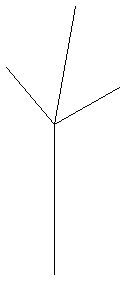
\includegraphics[width=0.15\textwidth]{./inf/SEKII/06_Java_Rekursion/Aufgabe2_2-2.png}
   \captionof{figure}{Ein Farnwedel der Stufe 2}
\end{minipage}\hfill                  
\begin{minipage}[b]{0.6\textwidth}
  \centering
   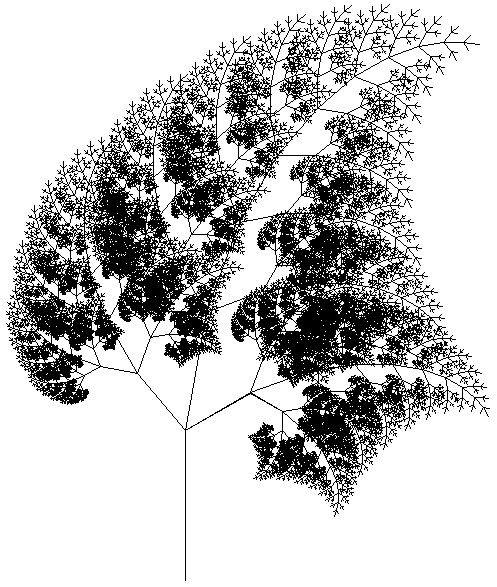
\includegraphics[width=0.5\textwidth]{./inf/SEKII/06_Java_Rekursion/Aufgabe2_2-11.png}
   \captionof{figure}{Ein Farnwedel der Stufe 11}
\end{minipage}


\section{Rekursion mit Turtle-Grafik (Fortsetzung)}

Für die folgenden Aufgaben kopierst du dir die Datei
\myFile{Rekursion3.java} aus dem Kurs-Repository in dein eigenes Projekt (und
dort in das bereits existierende Package \myPackage{rekursion}).

\subsection{Aufgabe 1: Kochsche Kurve I}

\begin{minipage}{0.55\textwidth}
Die Turtle steht mit Blick nach rechts. Eine  Kochsche Kurve der Stufe 1 ist
eine einfache Linie.
\end{minipage}\hfill
\begin{minipage}{0.4\textwidth}
  \centering
  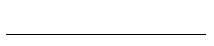
\includegraphics[width=1.0\textwidth]{./inf/SEKII/06_Java_Rekursion/Aufgabe3_1-1.png}
  \captionof{figure}{Kochsche Kurve Stufe 1}
\end{minipage}
% Abbildungen zu den Kochschen Kurven von http://www.oberstufeninformatik.de/
% "Die Materialien sind nicht Freeware, sondern Beerware. Voraussetzung für den
% Einsatz ist, dass der Benutzer ein Bier zum Wohle des Autors Horst Gierhardt 
% trinkt. Eine Flasche darf auch mit einem Roboter geöffnet werden. Über
% Rückmeldungen würde ich mich freuen!

\begin{minipage}{0.55\textwidth}
Eine Kochsche Kurve der Stufe 2 sieht wie rechts abgebildet aus. Die Linie wird
gedrittelt. Über dem Mittelstück wird ein gleichseitiges Dreieck angesetzt. Die
Seiten des Dreiecks sind alle ein Drittel der ursprünglichen Linie lang.

Überlege dir, wie groß der Innenwinkel des Dreiecks sein muss!
\end{minipage}\hfill
\begin{minipage}{0.4\textwidth}
  \centering
  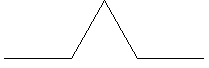
\includegraphics[width=1.0\textwidth]{./inf/SEKII/06_Java_Rekursion/Aufgabe3_1-2.png}
  \captionof{figure}{Kochsche Kurve Stufe 2}
\end{minipage}

\vspace{5mm}

\begin{minipage}[b]{1.0\textwidth}
  \centering
  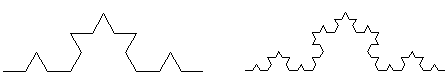
\includegraphics[width=0.8\textwidth]{./inf/SEKII/06_Java_Rekursion/Aufgabe3_1-34.png}
  \captionof{figure}{Kochsche Kurven der Stufe 3 und 4}
\end{minipage}

\vspace{5mm}

Programmiere zur Lösung der Aufgabe die Methode:

\begin{lstlisting}
public void koch(double laenge, int stufe)
\end{lstlisting}

Tipp: Nur bei Stufe 1 wird tatsächlich eine Linie gemalt. Kochsche Kurven einer
höheren Stufe, rufen zum „Zeichnen“ vier Mal rekursiv die Methode
\lstinline|koch()| mit einem Drittel von \lstinline|laenge| auf und drehen sich
zwischen den Aufrufen auf geeignete Weise.


\subsection{Aufgabe 2: Schneeflocke}

Die Turtle blickt zu Beginn nach oben. Drehe die Turtle um 30 Grad nach rechts
und rufe die Methode \lstinline|koch()| aus Aufgabe 1 mit der gewünschten
Anzahl Stufen auf. Drehe dich dann um 120 Grad nach rechts und rufe die Methode
\lstinline|koch()| erneut auf. Drehe dich ein zweites Mal um 120 Grad nach
rechts und rufe die Methode \lstinline|koch()| zum dritten Mal auf. Dadurch
werden drei Kochsche Kurven in Dreieck-Form hintereinander gehängt und man
erhält eine Art Schneeflocke.

\vspace{5mm}

\begin{minipage}[b]{1.0\textwidth}
  \centering
  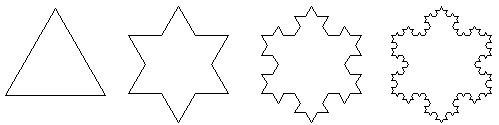
\includegraphics[width=0.8\textwidth]{./inf/SEKII/06_Java_Rekursion/Aufgabe3_2.png}
  \captionof{figure}{Kochsche Kurven werden zu Schneeflocken}
\end{minipage}



\subsection{Aufgabe 3: Variation zur Kochschen Kurve}

Der Ausgangspunkt ist derselbe wie in Aufgabe 2. Du sollst erneut drei Kochsche
Kurven in der Form eines Dreiecks anordnen, aber diesmal sollst du anders herum
gehen. Dadurch wird die Kochsche Kurve nicht nach außen sondern nach innen
entwickelt. Was für eine Figur entsteht?


\subsection{Aufgabe 4: Kochsche Kurve II}

Ordne vier Kochsche Kurven in Form eines Quadrats an. Zeichne das Quadrat so
herum, dass die Kochschen Kurven stufenweise nach innen entwickelt werden. Was
für eine Figur entsteht?


\subsection{Aufgabe 5: Kochsche Kurve III}

\begin{minipage}[b]{0.5\textwidth}
Die Turtle blickt zu Beginn nach rechts. Zeichne eine erweiterte Kochsche
Kurve, bei der auf das gleichseitige Dreieck noch ein  zweites, umgedrehtes
gleichseitiges Dreieck drauf gesetzt wird. Es entsteht ein hübsches Dreieck mit
Schneeflocken-Muster.
\end{minipage}\hspace{2mm}
\begin{minipage}[b]{0.1\textwidth}
  \centering
  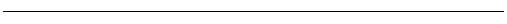
\includegraphics[width=1.0\textwidth]{./inf/SEKII/06_Java_Rekursion/Aufgabe3_5-1.png}
\end{minipage}\hspace{2mm}
\begin{minipage}[b]{0.15\textwidth}
  \centering
  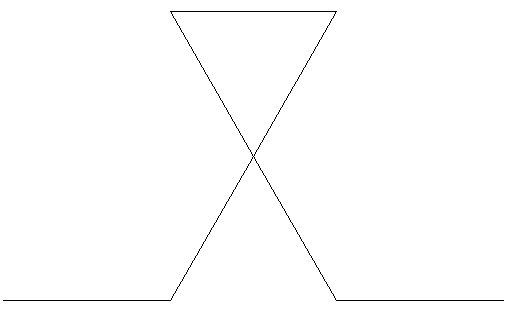
\includegraphics[width=1.0\textwidth]{./inf/SEKII/06_Java_Rekursion/Aufgabe3_5-2.png}
\end{minipage}\hspace{2mm}
\begin{minipage}[b]{0.2\textwidth}
  \centering
  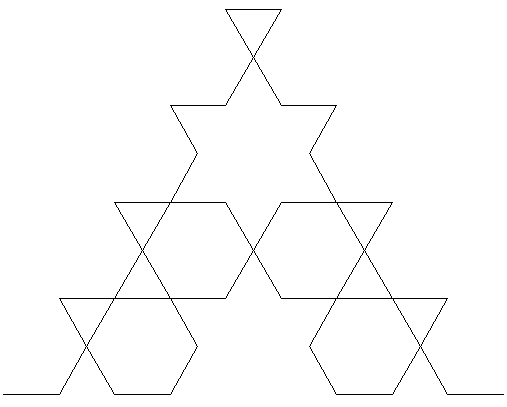
\includegraphics[width=1.0\textwidth]{./inf/SEKII/06_Java_Rekursion/Aufgabe3_5-3.png}
\end{minipage}


\subsection{Aufgabe 6: Sierpinski-Dreieck}
 
Ein Sierpinski-Dreieck der ersten Stufe besteht aus drei gleich langen
Strichen, die im 120° Winkel vom Mittelpunkt abgehen. In der 2.~Stufe wird am
Ende jedes Striches noch einmal die gleiche Figur angefügt, wobei die
Seitenlängen um die Hälfte verkürzt werden, usw.

\begin{minipage}{0.3\textwidth}
  \centering
  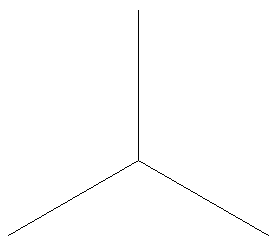
\includegraphics[width=0.7\textwidth]{./inf/SEKII/06_Java_Rekursion/Aufgabe3_6-1.png}
  \captionof{figure}{Stufe 1}
\end{minipage}\hfill
\begin{minipage}{0.3\textwidth}
  \centering
  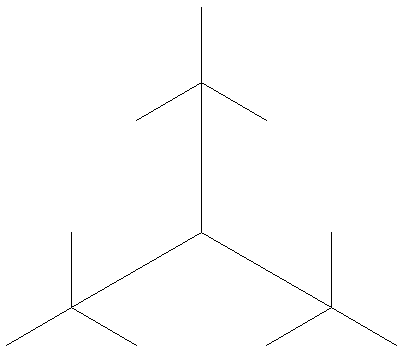
\includegraphics[width=0.7\textwidth]{./inf/SEKII/06_Java_Rekursion/Aufgabe3_6-2.png}
  \captionof{figure}{Stufe 2}
\end{minipage}

\begin{minipage}{1.0\textwidth}
  \centering
  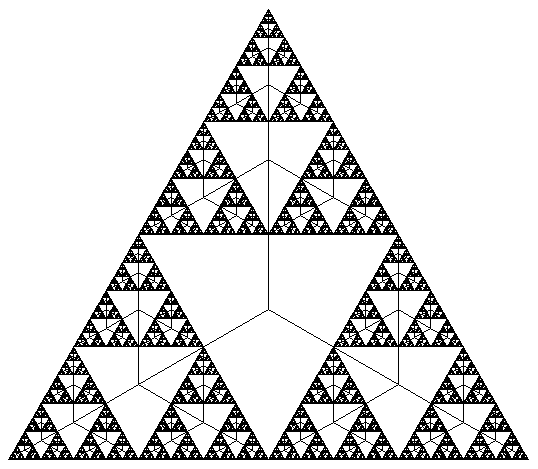
\includegraphics[width=0.5\textwidth]{./inf/SEKII/06_Java_Rekursion/Aufgabe3_6-10.png}
  \captionof{figure}{Sierpinski Dreieck Stufe 10}
\end{minipage}


\subsection{Aufgabe 7: Baum des Pythagoras}
 
Die Grundstruktur des „Baums des Pythagoras“ besteht aus einem Quadrat, über
dem ein rechtwinkliges Dreieck liegt. Auf jede Kathete des Dreiecks werden
wieder ein Quadrat und ein rechtwinkliges Dreieck gezeichnet, und so weiter.

Programmiere eine Methode

\begin{lstlisting}
public void pythagoras(double seite, int alpha, int stufe)
\end{lstlisting}

Durch den Aufruf 

\begin{lstlisting}
pythagoras(120, 35, 10);
\end{lstlisting}

soll ein Baum der Stufe 10 (beim Weg von der Wurzel bis zu einer Baumspitze
erscheinen 10 Quadrate) gezeichnet werden, dessen größtes Quadrat die
Seitenlänge 120 hat. Der Winkel Alpha im Dreieck sei 35 Grad groß.

\vspace{5mm}

\begin{minipage}{1.0\textwidth}
  \centering
  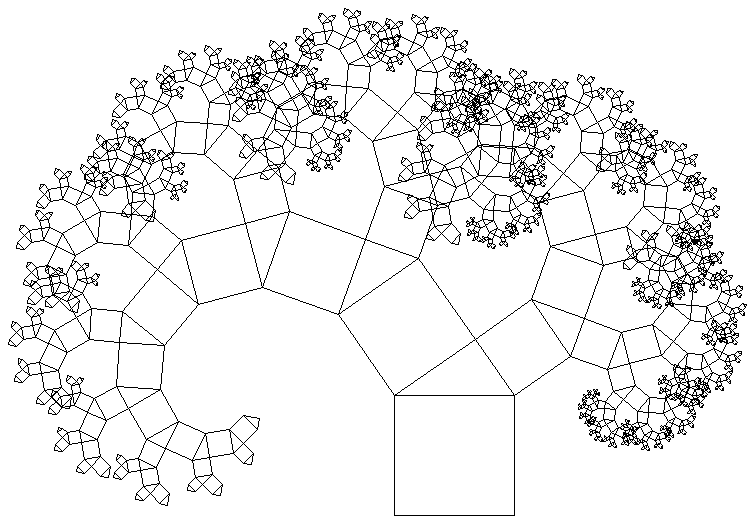
\includegraphics[width=0.9\textwidth]{./inf/SEKII/06_Java_Rekursion/Aufgabe3_7.png}
  \captionof{figure}{Baum des Pythagoras (10.\ Stufe)}
\end{minipage}\hfill